\documentclass{article}
\iffalse
This file is protected by Copyright. Please refer to the COPYRIGHT file
distributed with this source distribution.

This file is part of OpenCPI <http://www.opencpi.org>

OpenCPI is free software: you can redistribute it and/or modify it under the
terms of the GNU Lesser General Public License as published by the Free Software
Foundation, either version 3 of the License, or (at your option) any later
version.

OpenCPI is distributed in the hope that it will be useful, but WITHOUT ANY
WARRANTY; without even the implied warranty of MERCHANTABILITY or FITNESS FOR A
PARTICULAR PURPOSE. See the GNU Lesser General Public License for more details.

You should have received a copy of the GNU Lesser General Public License along
with this program. If not, see <http://www.gnu.org/licenses/>.
\fi

\author{} % Force author to be blank
%----------------------------------------------------------------------------------------
% Paper size, orientation and margins
%----------------------------------------------------------------------------------------
\usepackage{geometry}
\geometry{
	letterpaper,			% paper type
	portrait,				% text direction
	left=.75in,				% left margin
	top=.75in,				% top margin
	right=.75in,			% right margin
	bottom=.75in			% bottom margin
 }
%----------------------------------------------------------------------------------------
% Header/Footer
%----------------------------------------------------------------------------------------
\usepackage{fancyhdr} \pagestyle{fancy} % required for fancy headers
\renewcommand{\headrulewidth}{0.5pt}
\renewcommand{\footrulewidth}{0.5pt}
\rhead{\small{ANGRYVIPER Team}}
%----------------------------------------------------------------------------------------
% Appendix packages
%----------------------------------------------------------------------------------------
\usepackage[toc,page]{appendix}
%----------------------------------------------------------------------------------------
% Defined Commands & Renamed Commands
%----------------------------------------------------------------------------------------
\renewcommand{\contentsname}{Table of Contents}
\renewcommand{\listfigurename}{List of Figures}
\renewcommand{\listtablename}{List of Tables}
\newcommand{\todo}[1]{\textcolor{red}{TODO: #1}\PackageWarning{TODO:}{#1}} % To do notes
\newcommand{\code}[1]{\texttt{#1}} % For inline code snippet or command line
%----------------------------------------------------------------------------------------
% Various pacakges
%----------------------------------------------------------------------------------------
\usepackage{hyperref} % for linking urls and lists
\usepackage{graphicx} % for including pictures by file
\usepackage{listings} % for coding language styles
\usepackage{rotating} % for sideways table
\usepackage{pifont}   % for sideways table
\usepackage{pdflscape} % for landscape view
\usepackage{amsmath} % for equations
%----------------------------------------------------------------------------------------
% Table packages
%----------------------------------------------------------------------------------------
\usepackage{longtable} % for long possibly multi-page tables
\usepackage{tabularx} % c=center,l=left,r=right,X=fill
\usepackage{float}
\floatstyle{plaintop}
\usepackage[tableposition=top]{caption}
\newcolumntype{P}[1]{>{\centering\arraybackslash}p{#1}}
\newcolumntype{M}[1]{>{\centering\arraybackslash}m{#1}}
%----------------------------------------------------------------------------------------
% Block Diagram / FSM Drawings
%----------------------------------------------------------------------------------------
\usepackage{tikz}
\usetikzlibrary{shapes,arrows,fit,positioning}
\usetikzlibrary{automata} % used for the fsm
%----------------------------------------------------------------------------------------
% Colors Used
%----------------------------------------------------------------------------------------
\usepackage{colortbl}
\definecolor{blue}{rgb}{.7,.8,.9}
\definecolor{ceruleanblue}{rgb}{0.16, 0.32, 0.75}
\definecolor{drkgreen}{rgb}{0,0.6,0}
\definecolor{deepmagenta}{rgb}{0.8, 0.0, 0.8}
\definecolor{cyan}{rgb}{0.0,0.6,0.6}
\definecolor{maroon}{rgb}{0.5,0,0}
%----------------------------------------------------------------------------------------
% Update the docTitle and docVersion per document
%----------------------------------------------------------------------------------------
\def\docTitle{Component Data Sheet}
\def\docVersion{1.5}
%----------------------------------------------------------------------------------------
\date{Version \docVersion} % Force date to be blank and override date with version
\title{\docTitle}
\lhead{\small{\docTitle}}

\def\comp{pr\_cordic}
\edef\ecomp{pr_cordic}
\def\Comp{Polar to Rectangular CORDIC}
\graphicspath{ {figures/} }

\begin{document}

\section*{Summary - \Comp}
\begin{tabular}{|c|M{13.5cm}|}
	\hline
	\rowcolor{blue}
	                  &                                                              \\
	\hline
	Name              & \comp                                                        \\
	\hline
	Worker Type       & Application                                                  \\
	\hline
	Version           & v\docVersion \\
	\hline
	Release Date      & 4/2019 \\
	\hline
	Component Library & ocpi.assets.dsp\_comps                                        \\
	\hline
	Workers           & \comp.hdl                                                    \\
	\hline
	Tested Platforms  & xsim, isim, modelsim, alst4, ml605, ZedBoard(PL), Matchstiq-Z1(PL) \\
	\hline
\end{tabular}

\section*{Functionality}
\begin{flushleft}
	The {\Comp} component functions to perform a polar to rectangular conversion using a Coordinate Rotation Digital Computer (CORDIC) algorithm.
\end{flushleft}

\section*{Worker Implementation Details}
\subsection*{\comp.hdl}
Traditionally, CORDIC algorithms are represented with three inputs, $x_0$, $y_0$, and $z_0$	and their respective three outputs $x_N$, $y_N$, and $z_N$. For this polar to rectangular algorithm, we drive the $magnitude$ to $x_0$ and the $phase$ to $z_0$. This process is summarized below in Equation \ref{eq:inputsummary}.
\begin{equation} \label{eq:inputsummary}
	x_{0}=R, y_{0}=0, z_{0}=\theta
\end{equation}
Both the \textit{magnitude} and \textit{phase} are normalized prior to the CORDIC processes. The  \textit{magnitude} is normalized from $-1$ to $+1$ and the \textit{phase} is normalized from $-\pi$ to $+\pi$. Due to the iterative nature of CORDIC algorithms, there is a gain factor $A_{n}$ that needs to be handled within the system. This system accounts for the gain in Equation \ref{eq:gain} internally by scaling the $magnitude$ by a Gain Correction Factor $K_c$ as seen in Equation \ref{eq:Kc}.
\begin{equation} \label{eq:gain}
	A_{n}=\prod_{n}\sqrt{1+2^{-2i}}
\end{equation}
\begin{equation}  \label{eq:Kc}
	K_{c}=\dfrac{1}{A_n}=\prod_{i=0}^Ncos(atan(2^{-i})), n=STAGES-1
\end{equation}
Additionally, the $phase$ input is prescaled internally by $S_c$ in Equation \ref{eq:Sc} to simplify the arithmetic. Once $S_c$ is applied to $\theta$ the input range will have a maximum negative value corresponding to $-\pi$ and a maximum positive value corresponding to $+\pi-\delta$, where $\delta$ is defined in Equation \ref{eq:delta}.
\begin{equation}  \label{eq:Sc}
	S_{c}=2^{(DATA\_WIDTH-1)}/\pi
\end{equation}
\begin{equation} \label{eq:delta}
	\delta = 2\pi/2^{(DATA\_WIDTH)}
\end{equation}
This worker implementation takes the inputs from Equation \ref{eq:inputsummary} and scales them by the gain adjustment and phase prescaled to yield Equation \ref{eq:updatedinput}.
\begin{equation} \label{eq:updatedinput}
	x_{0}=K_{c}R, y_{0}=0, z_{0}= S_{c}/ \theta
\end{equation}
Lastly, the expected outputs are found in Equation \ref{eq:outputs}.
\begin{equation} \label{eq:outputs}
	x_{N}=Rcos(\theta), y_{N}=Rsin(\theta), z_{N}=0
\end{equation}

\section*{Theory}
CORDIC algorithms are iterative algorithms used to calculate various trigonometric functions. This CORDIC algorithm specifically performs the conversion from the polar coordinate system to rectangular coordinate system. In polar coordinates, inputs to this component are the $radius$ (or $magnitude$) and the $angle$ $\theta$, and expected outputs in the rectangular coordinate system are $x$ and $y$. This process is summarized below in Equation \ref{eq:highlevelsummary}.
\begin{equation} \label{eq:highlevelsummary}
	R,\theta \rightarrow x,y
\end{equation}

\section*{Block Diagrams}
\subsection*{Top level}
\begin{center}
	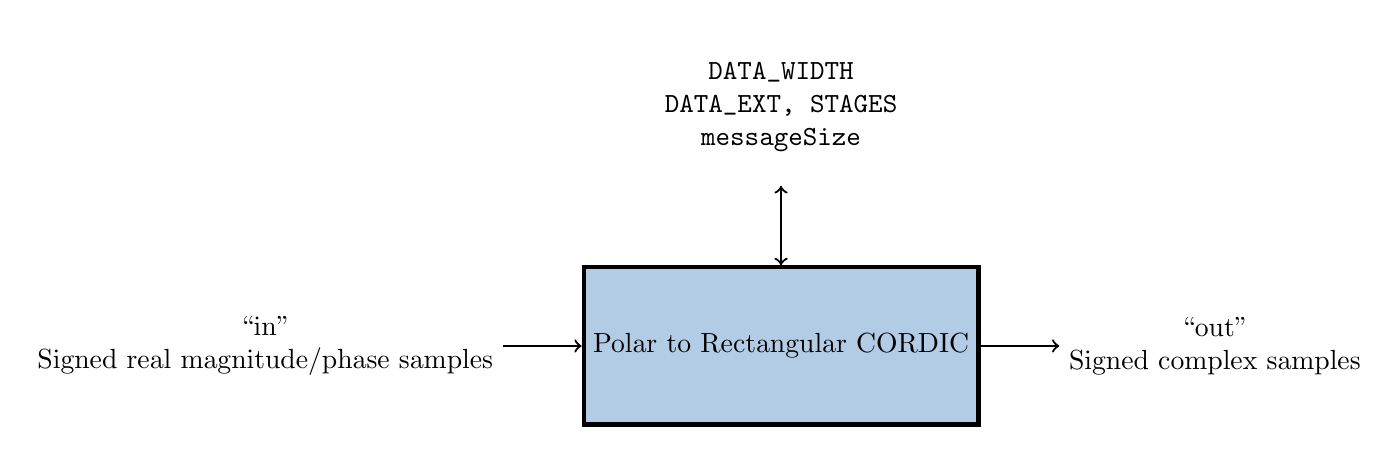
\begin{tikzpicture}[% List of styles applied to all, to override specify on a case-by-case
			every node/.style={
				align=center,  		% use this so that the "\\" for line break works
				minimum size=2cm	% creates space above and below text in rectangle
			},
			every edge/.style={draw,thick}
		]
		\node[rectangle,ultra thick,draw=black,fill=blue](R2){\Comp};
		\node[rectangle,draw=white,fill=white](R3)[left= of R2]{``in'' \\ Signed real magnitude/phase samples};
		\node[rectangle,draw=white,fill=white](R4)[right= of R2]{``out'' \\ Signed complex samples};
		\node[rectangle,draw=white,fill=white](R5)[above= of R2]{\verb+DATA_WIDTH+ \\ \verb+DATA_EXT, STAGES+ \\ \verb+messageSize+};
		\path[->]
		(R3)edge []	node [] {} (R2)
		(R2)edge []	node [] {} (R4)
		(R2)edge []	node [] {} (R5)
		(R5)edge []	node [] {} (R2)
		;
	\end{tikzpicture}
\end{center}

	\subsection*{State Machine}
	\begin{flushleft}
		Only one finite-state machine (FSM) is implemented by this worker. The FSM supports Zero-Length Messages.
	\end{flushleft}
	{\centering\captionsetup{type=figure}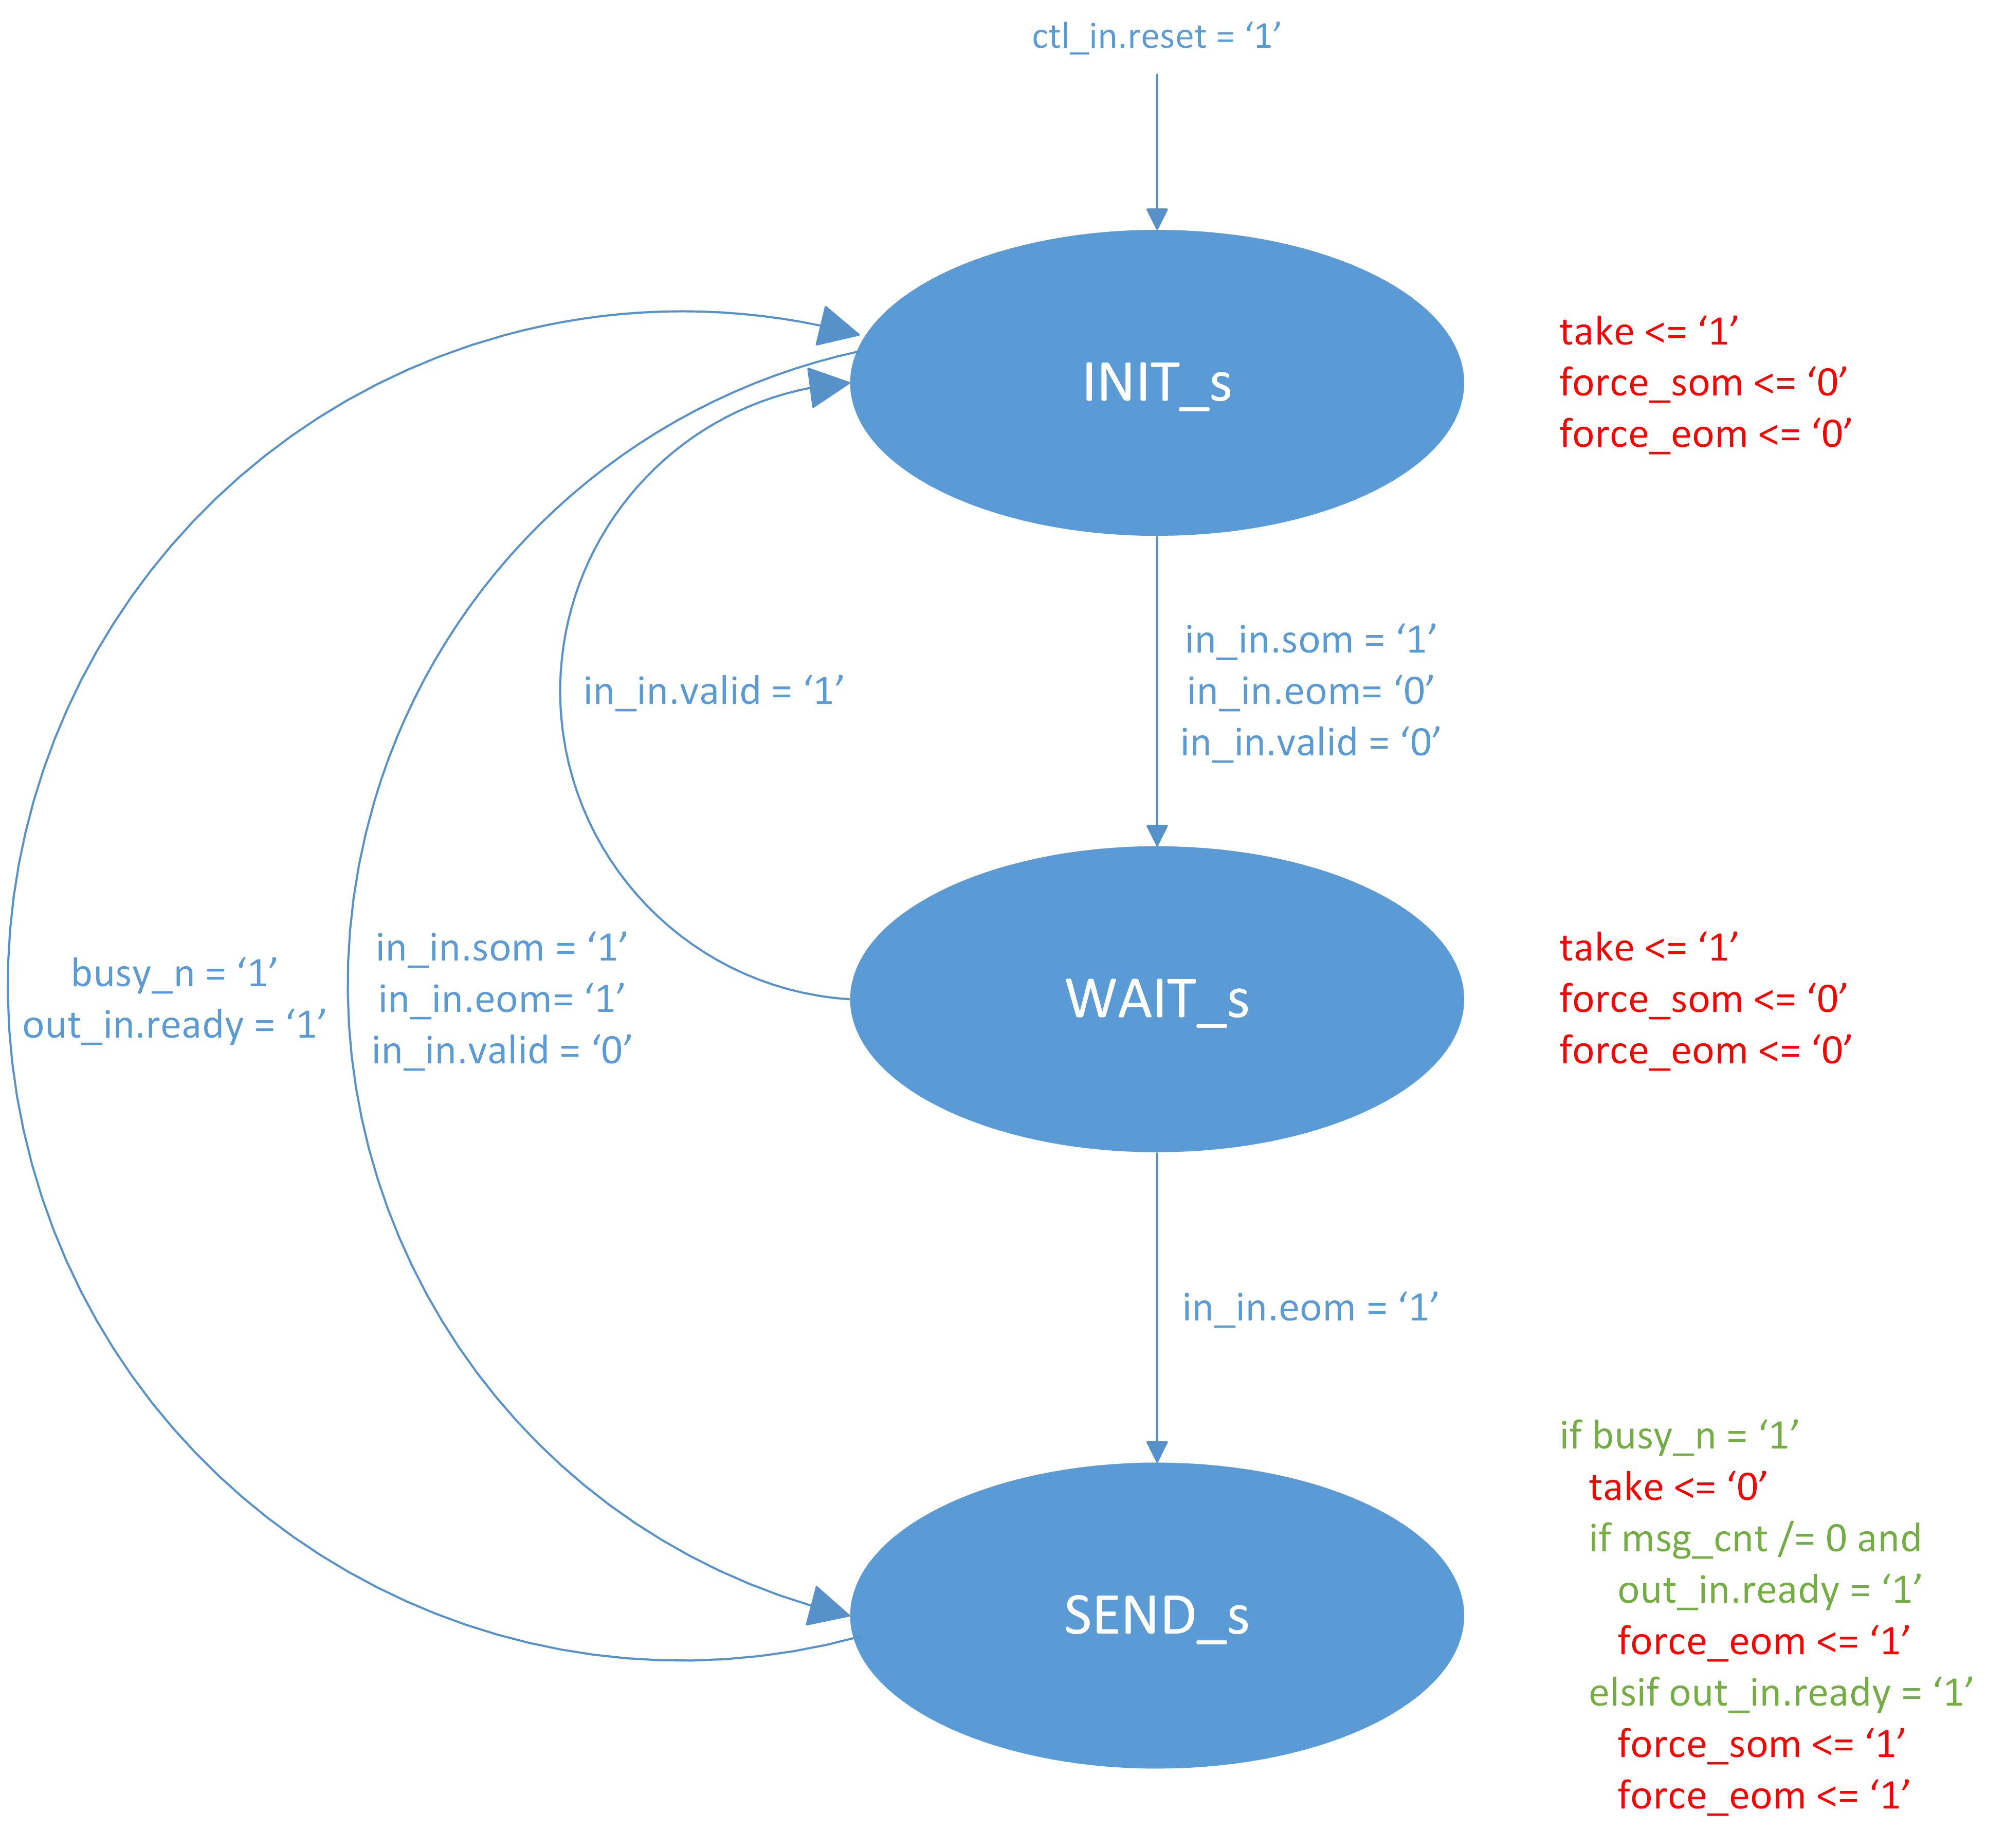
\includegraphics[scale=0.6]{zlm_fsm}\par\captionof{figure}{Zero-Length Message FSM}\label{fig:zlm_fsm}}
        \begin{flushleft}
	        Note: In future releases, this worker will be converted to the HDL version 2 API which will remove the need for this state machine.
        \end{flushleft}


\section*{Source Dependencies}
\subsection*{\comp.hdl}
\begin{itemize}
	\item projects/assets/components/dsp\_comps/pr\_cordic.hdl/pr\_cordic.vhd
	\item projects/assets/hdl/primitives/dsp\_prims/dsp\_prims\_pkg.vhd
	      \subitem projects/assets/hdl/primitives/dsp\_prims/cordic/src/cordic\_pr.vhd
	      \subitem projects/assets/hdl/primitives/dsp\_prims/cordic/src/cordic.vhd
	      \subitem projects/assets/hdl/primitives/dsp\_prims/cordic/src/cordic\_stage.vhd
\end{itemize}

\begin{landscape}
	\section*{Component Spec Properties}
	\begin{scriptsize}
		\begin{tabular}{|p{3cm}|p{1.5cm}|c|c|c|c|c|p{7cm}|}
			\hline
			\rowcolor{blue}
			Name                & Type   & SequenceLength & ArrayDimensions & Accessibility      & Valid Range & Default & Usage                                    \\
			\hline
			\verb+DATA_WIDTH+   & UChar  & -              & -               & Readable           & -           & -       & Real input and complex output data width \\
			\hline
			\verb+DATA_EXT+     & UChar  & -              & -               & Readable           & -           & -       & CORDIC requirement: \# of extension bits \\
			\hline
			\verb+STAGES+       & UChar  & -              & -               & Readable           & -           & -       & Number of CORDIC stages implemented      \\
			\hline
			\verb+messageSize+ & UShort & -              & -               & Writable, Readable & 8192        & 8192    & Number of bytes in output message        \\
			\hline
		\end{tabular}
	\end{scriptsize}

	\section*{Worker Properties}
	\subsection*{\comp.hdl}
	\begin{scriptsize}
		\begin{tabular}{|p{2cm}|p{1.5cm}|c|c|c|c|c|c|p{7cm}|}
			\hline
			\rowcolor{blue}
			Type         & Name              & Type & SequenceLength & ArrayDimensions & Accessibility & Valid Range & Default & Usage                                    \\
			\hline
			SpecProperty & \verb+DATA_WIDTH+ & -    & -              & -               & Parameter     & 1-16        & 16      & Real input and complex output data width \\
			\hline
			SpecProperty & \verb+DATA_EXT+   & -    & -              & -               & Parameter     & 1-16        & 16      & CORDIC requirement: \# of extension bits \\
			\hline
			SpecProperty & \verb+STAGES+     & -    & -              & -               & Parameter     & 16-32       & 16      & Number of CORDIC stages implemented      \\
			\hline
		\end{tabular}
	\end{scriptsize}

	\section*{Component Ports}
	\begin{scriptsize}
		\begin{tabular}{|M{2cm}|M{1.5cm}|M{4cm}|c|c|M{9cm}|}
			\hline
			\rowcolor{blue}
			Name & Producer & Protocol           & Optional & Advanced & Usage                  \\
			\hline
			in   & false    & iqstream\_protocol & false    & -        & Signed complex samples \\
			\hline
			out  & true     & iqstream\_protocol & false    & -        & Signed complex samples \\
			\hline
		\end{tabular}
	\end{scriptsize}

	\section*{Worker Interfaces}
	\subsection*{\comp.hdl}
	\begin{scriptsize}
		\begin{tabular}{|M{2cm}|M{1.5cm}|c|c|M{12cm}|}
			\hline
			\rowcolor{blue}
			Type            & Name & DataWidth & Advanced 					 & Usage                  \\
			\hline
			StreamInterface & in   & 32        & ZeroLengthMessages=true   & Signed magnitude samples (31:16), Signed phase samples (15:0) \\
			\hline
			StreamInterface & out  & 32        & ZeroLengthMessages=true   & Signed complex samples \\
			\hline
		\end{tabular}
	\end{scriptsize}
\end{landscape}

\section*{Control Timing and Signals}
\begin{flushleft}
	The CORDIC Polar-to-Rectangular HDL worker uses the clock from the Control Plane and standard Control Plane signals.
\end{flushleft}

\begin{landscape}
\section*{Worker Configuration Parameters}
\subsubsection*{\comp.hdl}
\input{../../\ecomp.hdl/configurations.inc}
\section*{Performance and Resource Utilization}
\subsubsection*{\comp.hdl}
\input{../../\ecomp.hdl/utilization.inc}
\end{landscape}
\section*{Test and Verification}
\begin{flushleft}
	A single test case is implemented to validate the CORDIC Polar-to-Rectangular component. An input file is generated with a constant magnitude of 29760 in bits (31:16) (driven into CORDIC input $x_0$) and two cycles of ramp data centered about zero representing a constant phase in bits (15:0) (driven into CORDIC input $z_0$). The expected outputs are a cosine from $I$ (the CORDIC $x_N$ output) with a magnitude equal to that of $x_0$ and a sine from $Q$ (the CORDIC $y_N$ output) also with a magnitude equal to that of $x_0$. Input magnitude and phase plots may be viewed in Figures \ref{fig:input_magnitude} and \ref{fig:input_phase} below.
\end{flushleft}

	\begin{figure}[ht]
		\centering
		\begin{minipage}{.5\textwidth}
			\centering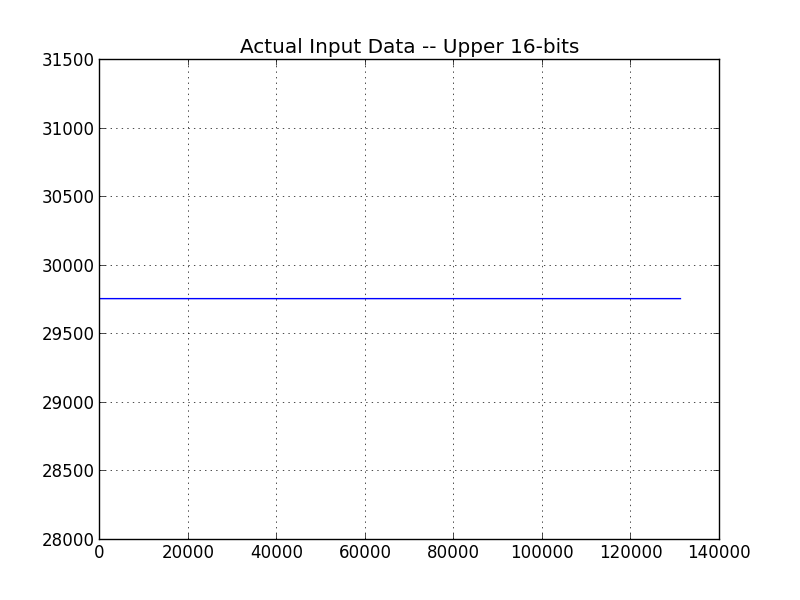
\includegraphics[width=1.0\linewidth]{input_magnitude}
			\captionof{figure}{Time Domain Magnitude Input}
			\label{fig:input_magnitude}
		\end{minipage}%
		\begin{minipage}{.5\textwidth}
			\centering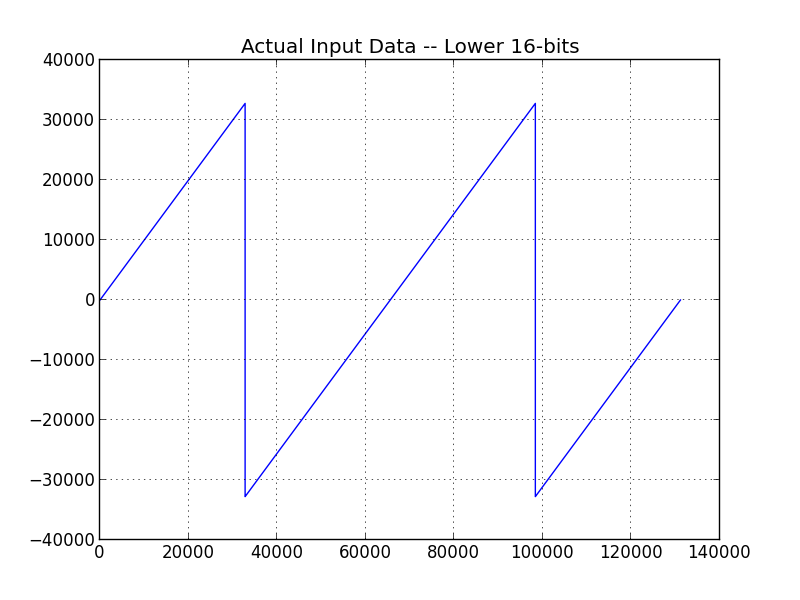
\includegraphics[width=1.0\linewidth]{input_phase}
			\captionof{figure}{Time Domain Phase Input}
			\label{fig:input_phase}
		\end{minipage}
	\end{figure}

\begin{flushleft}
	Verification of output data is performed by creating two cycles of a complex sinusoid in python, and then comparing the worker output sample-by-sample with these expected results. A difference of $\pm1.0$ is tolerated to allow for differences in fixed-point implementation and hardware rounding. Figures \ref{fig:output_time} and \ref{fig:output_freq} depict the output of the Polar to Rectangular CORDIC.
\end{flushleft}

	\begin{figure}[ht]
		\centering
		\begin{minipage}{.5\textwidth}
			\centering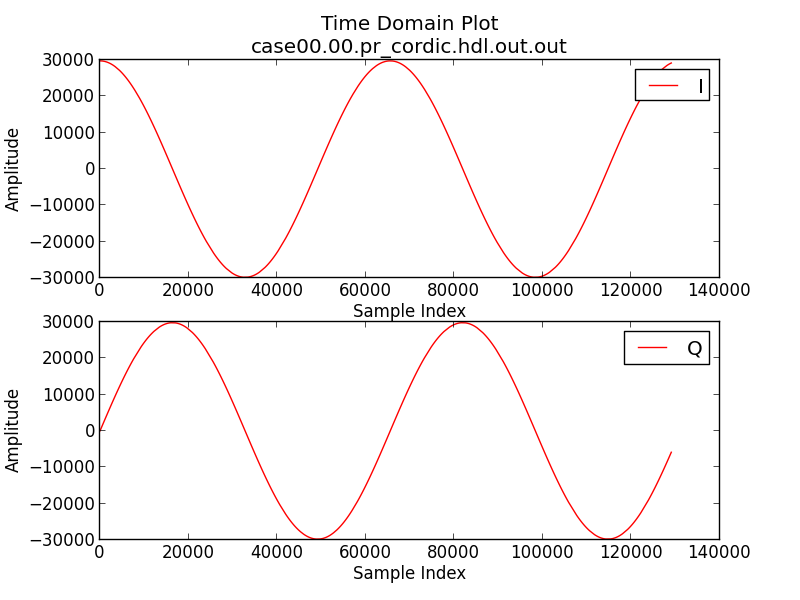
\includegraphics[width=1.0\linewidth]{output_time}
			\captionof{figure}{Time Domain Rectangular Output}
			\label{fig:output_time}
		\end{minipage}%
		\begin{minipage}{.5\textwidth}
			\centering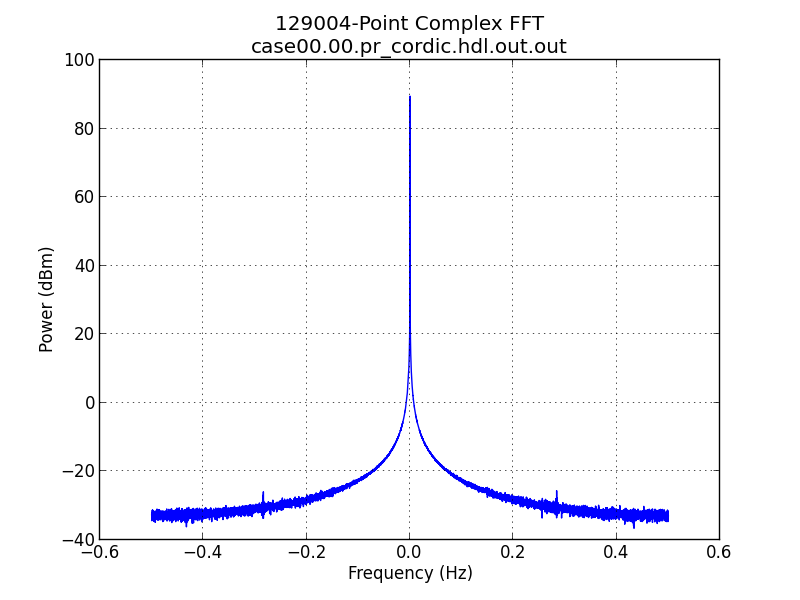
\includegraphics[width=1.0\linewidth]{output_freq}
			\captionof{figure}{Frequency Domain Rectangular Output}
			\label{fig:output_freq}
		\end{minipage}
	\end{figure}

\end{document}
